%TODO
%\subsection{Lista Consolidada}

%TODO
%\subsection{Tabelas de Seleção}

%TODO
%\subsection{Cache e Fecho Transitivo}

%TODO
%\section{\acrshort{rest}}
%~\cite{restws}

%TODO
%\section{express}
%\cite{wdmongo}
%procurar "semelhantes" para cada um

\section{\acrfull{jwt}}
O \acrshort{jwt} é um \textit{open standard}\footnote{Mais informação em \url{https://tools.ietf.org/html/rfc7519}} que define uma forma compacta e independente de transmitir com segurança informação entre partes com um objeto \acrshort{json}.~\cite{jwtio} O \acrshort{jwt} pode ser assinado digitalmente (\acrshort{jws}), encriptado (\acrshort{jwe}), assinado e depois encriptado (\acrshort{jws} encriptado, ou seja, um \acrshort{jwe}, ordem recomendada\footnote{Mais informação em \url{https://tools.ietf.org/html/rfc7519\#section-11.2}}) ou encriptado e depois assinado (\acrshort{jwe} assinado, ou seja, um \acrshort{jws}).

Caso seja assinado digitalmente é possível verificar a integridade da informação mas não é garantida a sua privacidade contudo podemos confiar na informação do \acrshort{jwt}. A assinatura pode ser efetuada através de um segredo usando por exemplo o algoritmo \acrshort{hmac} ou através de pares de chaves pública/privada usando por exemplo o algoritmo \acrshort{rsa}. No caso de se usar pares de chaves pública/privada a assinatura também garante que a parte envolvida que tem a chave privada é aquela que assinou o \acrshort{jwt}.

Por outro lado, os \acrshort{jwt}s podem ser encriptados garantindo a privacidade destes, escondendo a informação das partes não envolvidas. Nesta secção apenas se falará sobre \acrshort{jwt}s e \acrshort{jws}s (\acrshort{jwt} assinado). Se pretender saber mais sobre \acrshort{jwe}s pode ler o capítulo 5 do livro \textit{The JWT Handbook} por \textit{Sebastián E. Peyrott}.

Sendo assim em que casos é útil o uso de \acrshort{jwt}s? Dois dos casos são os seguintes:
\begin{itemize}
    \item Autorização: Este será o caso para o qual o \acrshort{jwt} será usado na \acrshort{clav}. Quando o utilizador realiza o \textit{login} gera-se um \acrshort{jwt} por forma a que os restantes pedidos desse utilizador sejam realizados com esse \acrshort{jwt} (\acrlong{sso}). O uso de \acrshort{jwt}s para estes casos permitem um \textit{overhead} pequeno e a flexibilidade de serem usados em diferentes domínios.
    \item Troca de informação: No caso de troca de informação entre duas partes os \acrshort{jwt}s assinados são de bastante utilidade visto que permitem verificar se o conteúdo não foi violado e, no caso de se usar pares de chaves pública/privada para assinar, permitem ter a certeza que o remetente é quem diz ser.
\end{itemize}

\subsection{Estrutura do \acrshort{jwt}}

Os \acrshort{jwt}s são construídos a partir de três elementos, o \textit{header} (objeto \acrshort{json} também conhecido por \acrshort{jose} \textit{header}), o \textit{payload} (objeto \acrshort{json}) e os dados de assinatura/encriptação (depende do algoritmo usado). Estes elementos são depois codificados em representações compactas (\texttt{Base64 URL-safe}\footnote{Variante da codificação \texttt{Base64} onde a codificação gerada é segura para ser usada em \textit{URL}s. Basicamente para a codificação \texttt{Base64} gerada substitui os caracteres '+' e '/' pelos caracteres '-' e '\_' respetivamente. Além disso, remove o caractere de \textit{padding} e proíbe separadores de linha}). As codificações \texttt{Base64 URL-safe} de cada elemento são depois concatenadas através de pontos dando origem a uma representação final compacta do \acrshort{jwt} (\textit{JWS/JWE Compact Serialization}). Na secção~\ref{sec:criacaojwt} está presente dois diagramas referentes à construção de dois \acrshort{jwt}s sendo um deles assinado.

\begin{figure}[H]
    \centering
    \textbf{\textcolor{red}{eyJhbGciOiJIUzI1NiIsInR5cCI6IkpXVCJ9}.
        \textcolor{purple}{eyJuYW1lIjoiSm9zw6kgTWFydGlucyIsIm51bSI6ImE3ODgyMSJ9}.
        \textcolor{cyan}{tRPSYVsFI-nziRPuAjdGZLN2tUez5MtLML\_aAnPplgM}
    }
    \caption{Exemplo de representação compacta de \acrshort{jwt} (quebra de linhas por forma a melhorar leitura)}\label{fig:exemjwt}
\end{figure}

De seguida vamos aprofundar cada elemento referido:
\begin{itemize}
    \item[\textbf{\textit{Header}:}]

    O cabeçalho (a vermelho na figura~\ref{fig:exemjwt}) consiste nos seguintes atributos:
    \begin{itemize}
        \item O atributo obrigatório (único campo obrigatório para o caso de um \acrshort{jwt} não encriptado) \texttt{alg} (algoritmo) onde é indicado que algoritmo é usado para assinar e/ou desencriptar. O seu valor pode ser por exemplo HS256 (\acrshort{hmac} com o auxilio do SHA-256\footnote{Função pertencente ao conjunto de funções \textit{hash} criptográficas \acrfull{sha2} desenhadas pela \acrshort{nsa}}) ou \acrshort{rsa}.
        \item O atributo opcional \texttt{typ} (tipo do \textit{token}) em que o seu valor é ``JWT''. Serve apenas para distinguir os \acrshort{jwt}s de outros objetos que têm um \acrshort{jose} \textit{header}.
        \item O atributo opcional \texttt{cty} (tipo do conteúdo (\textit{payload})). Se o \textit{payload} conter atributos arbitrários este atributo não deve ser colocado. Caso o \textit{payload} seja um \acrshort{jwt}\footnote{\acrshort{jwt} aninhado (\textit{nested \acrshort{jwt}})} então este atributo deve ter o valor de ``JWT''.
    \end{itemize}

    O cabeçalho é de grande importância visto que permite saber se o \acrshort{jwt} é assinado ou encriptado e de que forma o resto do \acrshort{jwt} deve ser interpretado.

    \begin{lstlisting}[language=json, caption=\textit{Header} usado para construir o \acrshort{jwt} da figura~\ref{fig:exemjwt}]
    {
        "alg": "HS256",
        "typ": "JWT"
    }
    \end{lstlisting}

    \item [\textbf{\textit{Payload}:}] O \textit{payload} (a roxo na figura~\ref{fig:exemjwt}) contém a informação/dados que pretendemos transmitir com o \acrshort{jwt}. Não há atributos obrigatórios contudo existem certos atributos que têm um significado definido (atributos registados).

    Existem 7 atributos registados (\textit{registered claims}):~\cite{jwthandbook}
    \begin{itemize}
        \item \texttt{iss} (\textit{issuer}): Identificador único (\textit{case-sensitive string}) que identifica unicamente quem emitiu o \acrshort{jwt}. A sua interpretação é específica a cada aplicação visto que não há uma autoridade central que gere os emissores.
        \item \texttt{sub} (\textit{subject}): Identificador único (\textit{case-sensitive string}) que identifica unicamente de quem é a informação que o \acrshort{jwt} transporta. Este atributo deve ser único no contexto do emissor, ou se tal não for possível, globalmente único. O tratamento do atributo é específico a cada aplicação. 
        \item \texttt{aud} (\textit{audience}): Identificador único (\textit{case-sensitive string}) ou \textit{array} destes identificadores únicos que identificam unicamente os destinatários pretendidos do \acrshort{jwt}. Ou seja, quem lê o \acrshort{jwt} se não estiver no atributo \texttt{aud} não deve considerar os dados contidos no \acrshort{jwt}. O tratamento deste atributo também é específico a cada aplicação. 
        \item \texttt{exp} (\textit{expiration (time)}): Um número inteiro que representa uma data e hora específica no formato \textit{seconds since epoch} definido pela \acrshort{posix}\footnote{Mais informação em \url{https://pubs.opengroup.org/onlinepubs/9699919799/basedefs/V1\_chap04.html\#tag\_04\_16}}, a partir da qual o \acrshort{jwt} é considerado inválido (expira).
        \item \texttt{nbf} (\textit{not before (time)}): Representa o inverso do atributo \texttt{exp} visto que é um número inteiro que representa uma data e hora específica no mesmo formato do atributo \texttt{exp}, mas que a partir da qual o \acrshort{jwt} é considerado válido.
        \item \texttt{iat} (\textit{issued at (time)}): Um número inteiro que representa uma data e hora especifica no mesmo formato dos atributos \texttt{exp} e \texttt{nbf} na qual o \acrshort{jwt} foi emitido.
        \item \texttt{jti} (\textit{\acrshort{jwt} ID}): Identificador único (\textit{string}) do \acrshort{jwt} que permite distinguir \acrshort{jwt}s com conteúdo semelhante. A implementação tem de garantir a unicidade deste identificador.
    \end{itemize}

    Estes atributos registados têm todos 3 caracteres visto que um dos requisitos do \acrshort{jwt} é ser o mais pequeno/compacto possível.

    Existem depois mais dois tipos de atributos, públicos e privados. Os atributos públicos podem ser definidos à vontade pelos utilizadores de \acrshort{jwt}s mas têm de ser registados em \textit{IANA JSON Web Token Claims registry} ou definidos por um espaço de nomes resistente a colisões de forma a evitar a colisão de atributos. Já os atributos privados são aqueles que não são nem registados nem públicos e podem ser definidos à vontade pelos utilizadores de \acrshort{jwt}s. Os dois atributos usados no exemplo~\ref{exem:pay} (\texttt{name} e \texttt{num}) são atributos privados.

    \begin{lstlisting}[language=json, caption=\textit{Payload} usado para construir o \acrshort{jwt} da figura~\ref{fig:exemjwt}, label=exem:pay]
    {
        "name": "José Martins",
        "num": "a78821"
    }
    \end{lstlisting}

\item [\textbf{\textit{Signature}:}] A assinatura (a azul na figura~\ref{fig:exemjwt}) é criada ao usar o algoritmo indicado na \textit{header} no atributo \texttt{alg} tendo como um dos argumentos os elementos codificados da \textit{header} e do \textit{payload} juntos por um ponto e como outro argumento um segredo. O resultado do algoritmo é depois codificado em \texttt{Base64 URL-safe}. Esta assinatura no caso dos \acrshort{jws}s é usada para verificar a integridade do \acrshort{jwt} e caso seja assinado com uma chave privada permite também verificar se o remetente é quem diz ser. No caso de o atributo \texttt{alg} for \texttt{none} a assinatura é uma \texttt{string} vazia.

    \begin{lstlisting}[language=javascript, caption=\textit{Signature} usado para construir o \acrshort{jwt} da figura~\ref{fig:exemjwt}]
    HMACSHA256(
        base64UrlEncode(header) + "." +
        base64UrlEncode(payload),
        segredo1.-uminho!clav
    )
    \end{lstlisting}
\end{itemize}

\subsection{Criação de \acrshort{jwt}/\acrshort{jws}}\label{sec:criacaojwt}

Na figura~\ref{fig:buildJWT} é apresentada a construção de um \acrshort{jwt} em que o atributo \texttt{alg} (algoritmo) tem o seu valor igual a \texttt{none}, ou seja, o \acrshort{jwt} não é assinado nem encriptado.

\begin{figure}[H]
    \begin{center}
        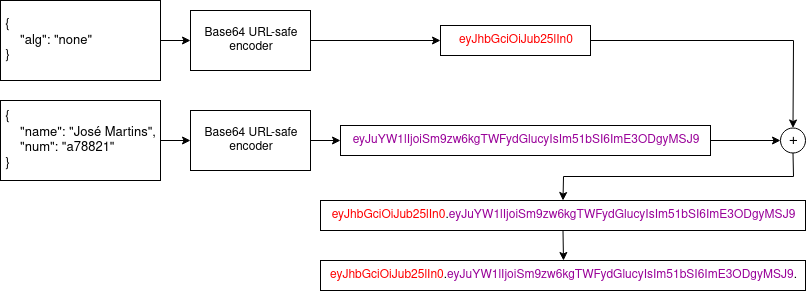
\includegraphics[width=1\textwidth]{img/buildJWT.png}
    \end{center}
    \caption{Criação de um \acrshort{jwt}}\label{fig:buildJWT}
\end{figure}

Já na figura~\ref{fig:buildJWS} é demonstrada a construção de um \acrshort{jwt} assinado, ou seja, um \acrshort{jws}.

\begin{figure}[H]
    \begin{center}
        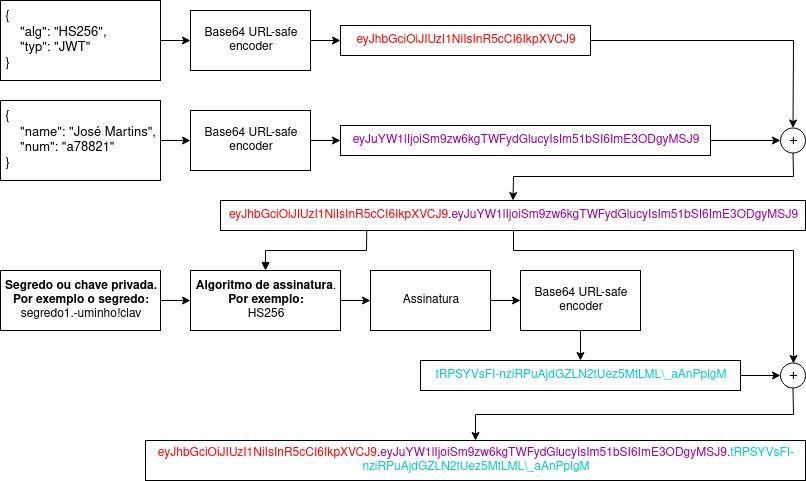
\includegraphics[width=1\textwidth]{img/buildJWS.png}
    \end{center}
    \caption{Criação de um \acrshort{jws}}\label{fig:buildJWS}
\end{figure}

\subsection{Alternativas ao \acrshort{jwt}}

Algumas alternativas ao \acrshort{jwt} passam pelo uso de \acrfull{swt} ou \acrfull{saml}. Se compararmos o \acrshort{jwt} ao \acrshort{saml}, o \acrshort{json} é menos verboso que o \acrshort{xml} e mesmo quando codificado o seu tamanho é menor. 

De um ponto de vista de segurança o \acrshort{swt} apenas pode ser assinado simetricamente por um segredo partilhado usando o algoritmo \acrshort{hmac}. Já o \acrshort{jwt} e o \acrshort{saml} podem usar pares de chaves pública/privada para assinar. Contudo assinar \acrshort{xml} com \textit{\acrshort{xml} Digital Signature} sem introduzir buracos de segurança é mais difícil quando comparado com a simplicidade de assinar \acrshort{json}.~\cite{jwtio}

Houve contudo algumas bibliotecas de \acrshort{jwt} com vulnerabilidades devido ao atributo \texttt{alg} da \textit{header} do \acrshort{jwt}. Havia duas situações de vulnerabilidade:
\begin{itemize}
    \item As bibliotecas ao fazer a verificação (recebe um \acrshort{jwt} e um segredo/chave pública como argumentos) de um \acrshort{jwt} com \texttt{alg} igual a \texttt{none} assumiam logo que o \acrshort{jwt} era válido mesmo que o segredo/chave pública fosse diferente de vazio. Ou seja, com a simples alteração do atributo \texttt{alg} e com a remoção da \textit{signature} podia-se alterar o \textit{payload} do \acrshort{jwt} que o servidor iria continuar a considerar que a integridade do \acrshort{jwt} não foi colocada em causa mesmo que os \acrshort{jwt}s gerados pelo servidor tivessem sido com um algoritmo e com recurso a um segredo/chave privada.
    \item As bibliotecas ao fazer a verificação seja um algoritmo simétrico ou assimétrico apenas tinham como parâmetros o \acrshort{jwt} e o segredo/chave pública. Isto gera uma segunda vulnerabilidade, se o servidor estiver à espera de um \acrshort{jwt} assinado com pares de chaves pública/privada mas recebe um \acrshort{jwt} assinado com \acrshort{hmac} vai assumir que a chave pública é o segredo a usar no algoritmo \acrshort{hmac}. Ou seja, se se criar um \acrshort{jwt} com o atributo \texttt{alg} igual a \acrshort{hmac} e a assinatura for gerada usando o algoritmo \acrshort{hmac} com o segredo a ser a chave pública, podemos alterar o \textit{payload} (antes de assinar) que o servidor vai considerar que o \acrshort{jwt} não foi maliciosamente alterado.
\end{itemize}

Portanto a flexibilidade de algoritmos dada pelo \acrshort{jwt} coloca em causa a segurança pelo que da parte das bibliotecas o atributo \texttt{alg} não deve ser considerado~\cite{jwtvuln} bem como deve ser \textit{deprecated} e deixar de ser incluído nos \acrshort{jwt}s\footnote{Ver \url{https://gist.github.com/paragonie-scott/c88290347c2589b0cd38d8bb6ac27c03}}. 

A biblioteca que será usada na \acrshort{clav}, \texttt{jsonwebtoken}\footnote{Ver \url{https://www.npmjs.com/package/jsonwebtoken}}, já endereçou estes problemas\footnote{Ver \url{https://github.com/auth0/node-jsonwebtoken/commit/1bb584bc382295eeb7ee8c4452a673a77a68b687}} pelo que estas vulnerabilidades não estarão presentes na \acrshort{clav}.

Ainda comparando as diferentes alternativas, os \textit{parsers} de \acrshort{json} são mais comuns em grande parte das linguagens de programação visto que os \acrshort{json}s mapeiam diretamente para objetos ao contrário do \acrshort{xml} que não tem um mapeamento natural de documento para objeto.~\cite{jwtio} Portanto isto torna mais fácil trabalhar com \acrshort{jwt} do que com \acrshort{saml}.

Já quando comparamos os \acrshort{jwt}s a \textit{cookie sessions}, o \acrshort{jwt} tem a vantagem de as sessões puderem ser \textit{stateless} enquanto que as \textit{cookies} são \textit{statefull}. Contudo, ser \textit{stateless} não permite por exemplo que a qualquer altura se possa revogar um \acrshort{jwt}. Para endereçar esse problema é necessário, por exemplo, guardar (\textit{statefull}) os \acrshort{jwt}s numa base de dados associando cada \acrshort{jwt} ao identificador único de quem é a informação contida no \acrshort{jwt} (o uso de uma \textit{whitelist}). Assim para revogar um \acrshort{jwt} bastaria removê-lo da base de dados.

Outra alternativa ao \acrshort{jwt} seria \textit{sessionIDs}. As \textit{sessionIDs} são \textit{strings} longas, únicas e aleatórias. É possível revogar um \textit{sessionID}, ao contrário do \acrshort{jwt}, bastando para isso remover o \textit{sessionID} da base de dados.

Por fim, uma outra alternativa bastante semelhante ao \acrshort{jwt} é \textit{Branca}. \textit{Branca} usa o algoritmo simétrico \textit{\acrshort{ietf} XChaCha20-Poly1305 \acrshort{aead}} que permite criar \textit{tokens} encriptados e que garantem integridade. Tem também uma região de \textit{payload} como \acrshort{jwt} com a única diferença é que este \textit{payload} não tem um estrutura definida. Não necessita da \textit{header} visto que o algoritmo usado não varia. Em vez de usar codificação em \texttt{Base64 URL-safe} usa \texttt{Base62} que também é \textit{URL-safe}. Para além disso o \textit{token} gerado é geralmente de menor dimensão do que o gerado pelo \acrshort{jwt} sendo como tal mais compacto que o \acrshort{jwt}.~\cite{branca} Visto que o \textit{Branca} encripta e garante integridade de uma forma mais simples que o \acrshort{jwt} permite (para isso era necessário recorrer a um \acrshort{jwe} que tem no seu \textit{payload} um \acrshort{jws}), sendo como tal propenso a menos erros de programação. Contudo, o \textit{Branca} ainda não é muito conhecido nem um \textit{standard} da indústria, ao contrário do \acrshort{jwt}, mas não deixa de ser algo a ter em conta para o futuro. 

%TODO
%\section{CORS}
%falar da package e do conceito CORS
%procurar "semelhantes" para cada um

%TODO
%\section{axios}
%procurar "semelhantes" para cada um

%TODO
%\section{HTTP Status}

%TODO
%\section{Headers do HTTP}

\section{Autenticação.gov}
O Autenticação.gov surgiu da necessidade de identificação unívoca de um utilizador perante sítios na Web.~\cite{agov} Será esta quem realiza o processo de autenticação do utilizador e que fornecerá os atributos do utilizador necessários para identificar o utilizador numa entidade (\textit{website}/portal).

O \acrshort{cc} em conjunto com o Autenticação.gov permite obter os identificadores dos utilizadores junto das entidades participantes da iniciativa do \acrshort{cc} (funcionalidade de Federação de Identidades da Plataforma de Interoperabilidade da Administração Pública). Além disso, o Autenticação.gov gere os vários fornecedores de atributos disponíveis bem como possui uma estreita ligação com a infraestrutura de chave pública do Cartão de Cidadão (\acrfull{pki}), com o intuito de manter os elevados níveis de segurança e privacidade no processo de autenticação e identificação.~\cite{agov}

O Autenticação.gov permite também a criação de credencias comuns a todos os sites da \acrshort{ap}, ou seja, o utilizador apenas necessita de se autenticar uma vez que poderá aceder aos vários portais (Portal do Cidadão, etc) com a mesma autenticação.

Para além disso o utilizador pode autenticar-se utilizando outros certificados digitais que não o \acrshort{cc} (por exemplo \acrfull{cmd}, \textit{user+password} ou redes sociais, estes dois últimos quando o \textit{website}/portal necessita apenas de conhecer do utilizador o \textit{email}).

No projeto \acrshort{clav} irá ser implementado a autenticação com recurso ao Autenticação.gov através de dois certificados digitais diferentes:
\begin{itemize}
    \item \acrfull{cc}: Já se encontra implementado como referido na secção~\ref{sec:autenticacao}. A autenticação é realizada através da leitura do \acrshort{cc} (através de um leitor de cartões sendo necessário a instalação de \textit{software} do Autenticação.gov para proceder à leitura do \acrshort{cc}) e posterior inserção do \acrshort{pin} de autenticação recebido quando se cria/renova o \acrshort{cc}.
    \item \acrfull{cmd}: Um dos objetivos desta tese é a implementação da autenticação com recurso a este certificado digital. Com o \acrshort{cmd}, após o utilizador associar um número de telemóvel ao \acrshort{nic}, o utilizador pode autenticar-se com o número de telemóvel, o código \acrshort{pin} da \acrshort{cmd} e o código de segurança temporário enviado por \acrshort{sms}.
\end{itemize}

De forma a completar a figura~\ref{fig:authgov} apresenta-se de seguida o fluxo de pedidos efetuado entre a \acrshort{clav} e o Autenticação.gov de forma a autenticar um utilizador na \acrshort{clav}:~\cite{agov}
\begin{figure}[H]
    \begin{center}
        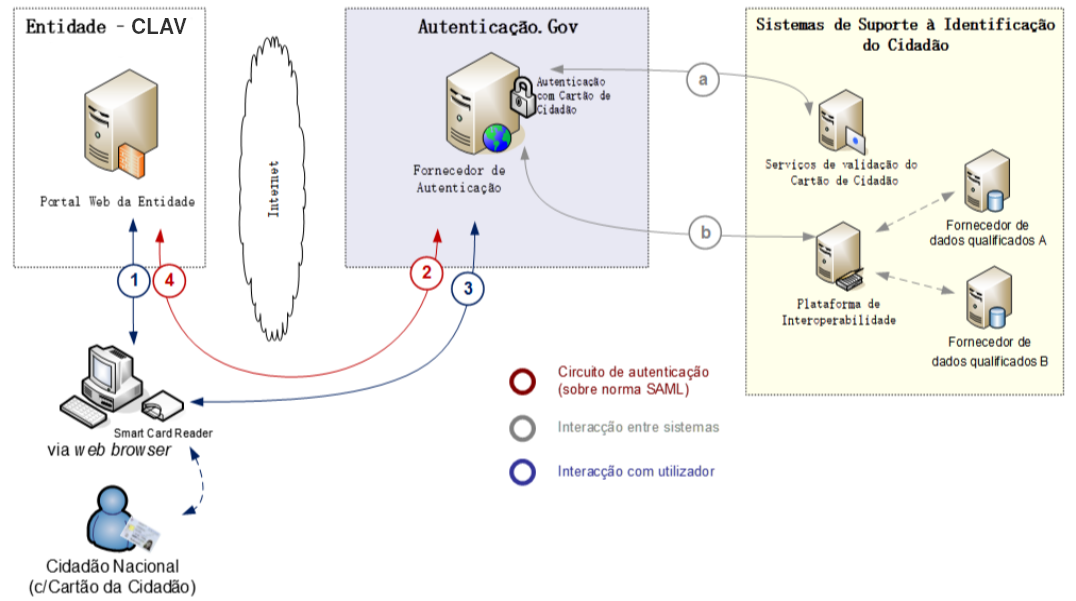
\includegraphics[width=1\textwidth]{img/fluxoauthgov.png}
    \end{center}
    \caption{Fluxo de pedidos entre a \acrshort{clav} e o Autenticação.gov de forma a autenticar um utilizador na \acrshort{clav}. Fonte:~\cite{agov}}\label{fig:fluxoauthgov}
\end{figure}

\begin{enumerate}
    \item O utilizador pretende aceder à área privada do portal de uma entidade (da \acrshort{clav}), na qual é necessário que comprove a sua identidade;
    \item O portal da entidade (\acrshort{clav}) delega a autenticação e redireciona o utilizador para o Autenticação.gov, juntamente com um pedido de autenticação assinado digitalmente;
    \item O Autenticação.gov valida o pedido de autenticação recebido e solicita a autenticação do utilizador com recurso ao seu \acrshort{cc} pedindo a inserção do seu \acrshort{pin} de autenticação. Durante este processo, o Autenticação.gov efetua as seguintes operações internas:
    \begin{enumerate}
        \item Valida as credenciais do utilizador com recurso à \acrshort{pki} do \acrshort{cc} via \acrshort{ocsp}
        \item Obtém atributos que sejam solicitados pelo portal da entidade (\acrshort{clav}) junto dos vários fornecedores de atributos qualificados. Esta operação é efetuada via Plataforma de Interoperabilidade. Este processo pode incluir a obtenção de dados da Federação de Identidades ou de outras Entidades.
    \end{enumerate}
    \item A identificação e atributos do utilizador são autenticadas e assinados digitalmente pelo Autenticação.gov, após o que redireciona o utilizador de volta ao portal da entidade original (\acrshort{clav}). Cabe à entidade (\acrshort{clav}) a validação das credenciais do Autenticação.gov e utilização dos atributos do cidadão.
\end{enumerate}

A troca de pedidos entre a \acrshort{clav} e o Autenticação.gov é feita através de \acrshort{saml} 2.0 (com as extensões que a \acrshort{ama} considera obrigatórias). De seguida será feita uma pequena introdução ao \acrshort{saml} 2.0. 

\subsection{\acrshort{saml} 2.0}
O \acrfull{saml} define uma \textit{framework} \textit{standard} em \acrshort{xml}.~\cite{sam2man} Foi aprovado pela \acrshort{oasis} e permite a troca segura de informação de autenticação e autorização entre diferentes entidades. Através do \acrshort{saml} é possível através de uma credencial (\textit{login} de um utilizador) aceder autenticado a um conjunto de \textit{websites}. Esta funcionalidade é conhecida por \acrfull{sso}.

Existem três tipos de papéis em \acrshort{saml}:~\cite{wisaml}
\begin{itemize}[leftmargin=2cm]
    \item Utilizador
    \item \textit{Identity Provider}: Realiza a autenticação de que o utilizador é quem diz ser e envia essa informação ao \textit{Service Provider} junta com as permissões de acesso do utilizador para o serviço
    \item \textit{Service Provider}: Precisa de autenticação do \textit{Identity Provider} para poder dar autorização ao utilizador
\end{itemize}

O documento \acrshort{xml} enviado pelo \textit{Identity Provider} para o \textit{Service Provider} é conhecida por \textit{\acrshort{saml} Assertion}. Existem três tipos de \textit{\acrshort{saml} Assertion}:~\cite{wisaml}
\begin{itemize}[leftmargin=2cm]
    \item \textit{Authentication Assertion}: Prova a identificação de um utilizador e fornece a hora em que o utilizador se autenticou e o método de autenticação usado
    \item \textit{Attribution Assertion}: Envia \textit{\acrshort{saml} attributes} (formato de dados que contém informação acerca do utilizador) para o \textit{Service Provider}
    \item \textit{Authorization Assertion}: Indica se o utilizador está autorizado a usar o serviço ou se o \textit{Identity Provider} recusou o pedido à inserção de uma password errada ou por falta de permissões para usar o serviço
\end{itemize}

No projeto \acrshort{clav} o utilizador final é o utilizador da \acrshort{clav}, o \textit{Identity Provider} é representado pelo Autenticação.gov e o \textit{Service Provider} é representado pela \acrshort{clav}.

%TODO
%\section{exceljs}
    %procurar "semelhantes" para cada um

%TODO
%\section{MongoDB}
%~\cite{wdmongo}

%TODO
%\section{mongoose}
%procurar "semelhantes" para cada um

\section{Swagger}
O \textit{Swagger} é um ecossistema de ferramentas para desenvolver \acrshort{api}s com a \acrfull{oas}.

Até 2015 o \textit{Swagger} consistia numa especificação e num ecossistema de ferramentas para implementar a especificação. Em 2015 a fundadora do \textit{Swagger}, \textit{SmartBear Software}, doou a especificação \textit{Swagger} para a \textit{Linux Foundation} e renomeou a especificação para \acrlong{oas}.~\cite{wiswagger}

A especificação \textit{OpenAPI} é agora desenvolvida pela \textit{OpenAPI Initiative} que envolve várias empresas tecnológicas entre as quais \textit{Microsoft}, \textit{Google}, \textit{IBM} e a fundadora \textit{Smartbear Software}.

Já o conjunto de ferramentas \textit{Swagger} inclui ferramentas \textit{open-source}, gratuitas e comerciais que podem ser usadas em diferentes estágios do ciclo de vida de uma \acrshort{api}, que inclui documentação, desenho, testes e \textit{deployment}. Algumas das ferramentas são:~\cite{swaggerVSoas}
\begin{itemize}
    \item \textbf{\textit{Swagger Editor}}: Permite editar especificações \textit{OpenAPI} em \acrshort{yaml} no \textit{browser}\footnote{Aceder \url{https://editor.swagger.io/}}, validar as especificações em relação às regras do \acrshort{oas} bem como pré-visualizar a documentação em tempo real. Facilita o desenho e a documentação de \acrshort{api}s \acrshort{rest}
    \item \textbf{\textit{Swagger \acrshort{ui}}}: Coleção de \textit{assets} \textit{\acrshort{html}}, \textit{JavaScript} e \textit{\acrshort{css}} que geram dinamicamente documentação a partir de uma especificação \textit{OpenAPI} de uma \acrshort{api}
    \item \textbf{\textit{Swagger Codegen}}: Permite a geração de bibliotecas cliente (geração de \acrshort{sdk}), \textit{server stubs} e documentação automática a partir de especificações \textit{OpenAPI}
    \item \textbf{\textit{Swagger Inspector}} (gratuita): Ferramenta de testes de \acrshort{api}s que permite validar as \acrshort{api}s e gerar definições \textit{OpenAPI} de \acrshort{api}s existentes
    \item \textbf{\textit{SwaggerHub}} (gratuita e comercial): Desenho e documentação de \acrshort{api}s, construído para equipas que trabalham com \textit{OpenAPI}
\end{itemize}

O \textit{Swagger} possui duas abordagens:~\cite{swaggerNode}
\begin{itemize}
    \item \textit{top-down}: Uso do \textit{Swagger Editor} para criar a especificação \textit{OpenAPI} e depois usar o \textit{Swagger Codegen} por forma a gerar o código do cliente e do servidor. Ou seja, primeiro desenha-se a \acrshort{api} antes de escrever código
    \item \textit{bottom-up}: Utilizador já possui uma \acrshort{api} \acrshort{rest} e o \textit{Swagger} irá ser usado apenas para documentar a \acrshort{api} existente
\end{itemize}

Visto que a \acrshort{clav} já possui grande parte da \acrshort{api} construída vai ser usada uma abordagem \textit{bottom-up}. Portanto, o \textit{Swagger} vai ser usado apenas para a documentação da \acrshort{api}. De forma a produzir a documentação, do portfólio de ferramentas do \textit{Swagger} apenas precisaremos de utilizar o \textit{Swagger \acrshort{ui}} e o \textit{Swagger Editor}. O primeiro permitirá apresentar aos utilizadores a documentação gerada e o segundo permitirá validar a especificação \textit{OpenAPI} (documentação) criada, verificando se não possui erros.

\subsection{Especificação \textit{OpenAPI}}

A especificação \textit{OpenAPI} providencia um conjunto de propriedades que podem ser usadas para descrever uma \acrshort{api} \acrshort{rest}. Com um documento de especificação válido é possível usá-lo para criar uma documentação interativa, por exemplo, através do \textit{Swagger \acrshort{ui}}.

De seguida será apresentado o que é possível documentar com a especificação \textit{OpenAPI} e como. É possível usar \acrshort{yaml} como \acrshort{json} para a especificar. Esta parte será demonstrada usando \acrshort{yaml}.\footnote{A especificação completa do \textit{OpenAPI} com versão igual a 3.0.0 pode ser vista em \url{https://github.com/OAI/OpenAPI-Specification/blob/master/versions/3.0.0.md}}

\subsubsection{Metadata}
O primeiro passo é escolher a versão da especificação \textit{OpenAPI} que irá ser usada para documentar:
\begin{lstlisting}[language=yaml, caption=Exemplo de indicação da versão da especificação \textit{OpenAPI}]
openapi: 3.0.0
\end{lstlisting}

Depois na secção \texttt{info} é possível descrever um pouco sobre a \acrshort{api} que estamos a documentar, indicando o título, a descrição e a versão da \acrshort{api}. As propriedades \texttt{title} e \texttt{version} são obrigatórias. É possível também colocar informação sobre os contactos disponíveis, termos de uso e a licença:\footnote{Ver mais em \url{https://github.com/OAI/OpenAPI-Specification/blob/master/versions/3.0.0.md\#infoObject}}
\begin{lstlisting}[language=yaml, caption={Exemplo de secção \texttt{info} indicando título, descrição e versão da \acrshort{api} na especificação \textit{OpenAPI}}]
info:
  title: CLAV API
  description: Esta é a API do projeto CLAV...
  version: 1.0.0
\end{lstlisting}

\vspace{-0.7cm}

\subsubsection{Servidores}
Há depois uma secção com o nome de \texttt{servers} para indicar os \textit{URL}s da \acrshort{api} que se pode aceder. Podem ser indicados mais do que um \textit{URL}:\footnote{Para mais detalhes sobre esta secção veja \url{https://swagger.io/docs/specification/api-host-and-base-path/}}
\begin{lstlisting}[language=yaml, caption=Exemplo de secção \texttt{servers} indicando os \textit{URL}s e a descrição de cada na especificação \textit{OpenAPI}]
servers:
  - url: http://clav-api.dglab.gov.pt/api
    description: Official API server
  - url: http://clav-test.di.uminho.pt/api
    description: Testing server
  - url: http://localhost:7779/api
    description: Local server
\end{lstlisting}

\vspace{-0.7cm}

\subsubsection{Caminhos/Rotas}
De seguida apresenta-se uma das secções mais importantes da especificação, a secção \texttt{paths}. Aqui são definidas as rotas que a \acrshort{api} disponibiliza. Para definir cada rota basta indicar o caminho relativo aos \acrshort{url}s definidos na secção \texttt{servers} (\verb|<server-url>/<caminho relativo>|). Nesta secção é definido tudo que envolve as rotas, desde os parâmetros necessários, as respostas que devolve, os métodos \textit{HTTP} disponíveis, etc:\footnote{Mais detalhes em \url{https://swagger.io/docs/specification/paths-and-operations/}}\footnote{mais detalhes sobre a funcionalidade \texttt{\$ref} em \url{https://swagger.io/docs/specification/using-ref/}}
\begin{lstlisting}[language=yaml, caption=Exemplo de secção \texttt{paths} indicando os detalhes de cada rota na especificação \textit{OpenAPI}, label={exem:oapiRota}]
paths:
  /users/{id}:
    get:
      summary: Resumo do que faz a rota
      description: >
        Descrição detalhada, pode ser usado Markdown para enriquecer o texto
      parameters:
        - name: id
          in: path
          description: Id do utilizador
          required: true
          schema:
            type: string
      responses:
        200:
          description: Descrição da resposta, p.e: Sucesso
          content:
            application/json:
              schema:
                #A estrutura do JSON devolvido pode ser definido logo aqui ou num componente à parte, fazendo referência desse. Iremos aplicar o segundo caso para demonstrar que estas funcionalidades tornam a documentação mais fácil de manter
                $ref: '#/components/schemas/User'
    post:
      ...
    delete:
      ...
  /users:
    ...

components:
  schemas:
    User:
      type: object
      properties:
        id:
          type: string
        ...
      required:
        - id
        ...
\end{lstlisting}

Outro ponto importante a referir é que é possível agrupar as rotas em grupos através do uso de \textit{tags}. As \textit{tags} tem de ser definidas numa secção chamada \textit{tags}:
\begin{lstlisting}[language=yaml, caption={Exemplo de secção \texttt{tags} defininfo tags na especificação \textit{OpenAPI}}]
tags:
  - name: users
    description: Descrição
  - name: classes
    description: Outra descrição
\end{lstlisting}

Depois em cada rota é necessário indicar a que \textit{tag} (grupo) pertence:
\begin{lstlisting}[language=yaml, caption=Exemplo de uso de \textit{tags} numa rota na especificação \textit{OpenAPI}]
paths:
  /users/{id}:
    get:
      summary: Resumo do que faz a rota
      tags:
        - users
      ...
\end{lstlisting}

\vspace{-0.7cm}

\subsubsection{Parâmetros}\label{sec:paramSwagger}
Como já exemplificado no exemplo~\ref{exem:oapiRota} os parâmetros de uma rota são definidos na secção \texttt{parameters} de cada rota. Existem quatro tipo de parâmetros que variam de acordo com o local onde se encontram. O tipo de um parâmetro é definido na propriedade \texttt{in} de um parâmetro e pode ser um dos seguintes:
\begin{itemize}
    \item Parâmetros no caminho: Servem normalmente para apontar para um recurso específico. Estes parâmetros são sempre obrigatórios como tal a propriedade \texttt{required} com o valor igual a verdadeiro deve ser sempre adicionado. Para além disso o \texttt{name} tem de ser igual ao que está no caminho. A propriedade \texttt{in} tem o valor de \textit{path}.
    \item Parâmetros na \textit{query string}: A propriedade \texttt{in} tem o valor de \textit{query}. No caso de tokens passados em parâmetros da \textit{query string} deve-se usar esquemas de segurança, veja a secção~\ref{sec:authSwagger} Autenticação.
    \item Parâmetros no cabeçalho: A propriedade \texttt{in} tem o valor de \textit{header}. Contudo os cabeçalhos \textit{Accept}, \textit{Content-Type} e \textit{Authorization} não são aqui definidos.
    \item Parâmetros no cabeçalho da \textit{Cookie}: A propriedade \texttt{in} tem o valor de \textit{cookie}.
\end{itemize}

Cada parâmetro tem várias propriedades que permitem defini-lo:\footnote{Mais detalhes em \url{https://swagger.io/docs/specification/describing-parameters/}}
\begin{itemize}
    \item \texttt{required}: Indica se o parâmetro é obrigatório ou opcional. Possíveis valores são \textit{true} ou \textit{false}.
    \item Na propriedade \texttt{schema}:
    \begin{itemize}
        \item \texttt{default}: Valor padrão de um parâmetro opcional
        \item \texttt{type}: O tipo do parâmetro. Possíveis valores: \textit{string}, \textit{integer}, etc
        \item \texttt{enum}: Indica os possíveis valores para o parâmetro
        \item \texttt{nullable}: Indica se o parâmetro pode ser \textit{null}. Possíveis valores são \textit{true} ou \textit{false}.
    \end{itemize}
    \item \texttt{allowEmptyValue}: Indica se o parâmetro pode ser vazio. Apenas aplicável no caso de um parâmetro na \textit{query string}. Possíveis valores são \textit{true} ou \textit{false}.
    \item \texttt{example}: Um exemplo do valor
    \item \texttt{examples}: Múltiplos exemplos
    \item \texttt{deprecated}: Indica se o parâmetro é ou não \textit{deprecated}. Possíveis valores são \textit{true} ou \textit{false}.
\end{itemize}

\subsubsection{\textit{Request Body}}
O \textit{request body} é definido em cada rota na secção \texttt{requestBody} sendo usado essencialmente em rotas com o método \acrshort{http} igual a POST ou a PUT, ou seja, em casos que há necessidade de criar ou alterar um objeto de acordo com a informação fornecida no pedido. As propriedades que podem ser definidas no \texttt{requestBody} são as seguintes:\footnote{Para mais detalhes, desde \textit{upload} de ficheiros, a \textit{Form Data}s, veja em \url{https://swagger.io/docs/specification/describing-request-body/}}\footnote{Para mais informação sobre os \textit{media types} veja \url{https://swagger.io/docs/specification/media-types/}}
\begin{itemize}
    \item \texttt{description}: Opcionalmente pode ser adicionada uma descrição
    \item \texttt{required}: Indica se o \textit{request body} é obrigatório ou opcional. Possíveis valores são \textit{true} ou \textit{false}. Por padrão o \textit{request body} é opcional.
    \item \texttt{content}: Obrigatório. Lista os \textit{media types} consumidos pela rota e especifica o \texttt{schema} para cada \textit{media type}
\end{itemize}

\subsubsection{Respostas}
Nesta secção, propriedade \texttt{responses} de cada rota, é descrita as possíveis respostas de cada rota. Na propriedade será definido as várias respostas, uma resposta por cada \acrshort{http} \textit{status code} possível de ser devolvido pela rota. Cada resposta pode possuir as seguintes propriedades:\footnote{Mais detalhes em \url{https://swagger.io/docs/specification/describing-responses/}}
\begin{itemize}
    \item \texttt{description}: Obrigatório, descrição da resposta
    \item \texttt{content}: Opcional, semelhante ao \texttt{content} do \textit{request body} e define o conteúdo que é devolvido.
    \item \texttt{headers}: Opcional, define as \textit{headers} que são devolvidas na resposta
\end{itemize}

\subsubsection{Adição de Exemplos}
Na secção~\ref{sec:paramSwagger} Parâmetros já se referiu como é possível adicionar exemplos aos parâmetros. De forma semelhante o mesmo pode ser realizado tanto no \textit{request body} como nas respostas através da propriedade \texttt{example} (um exemplo) ou \texttt{examples} (múltiplos exemplos) aninhado na propriedade \texttt{schema} ou aninhado na ``propriedade'' \textit{media type} no caso do \texttt{schema} ser uma referência para um modelo presente na secção \texttt{components}. A propriedade \texttt{example} pode também ser usada em objetos ou propriedades de um \texttt{schema}. Por fim, para adicionar exemplos de \acrshort{xml} ou \acrshort{html} os exemplos devem ser exemplificados como \textit{strings}:\footnote{Mais detalhes em \url{https://swagger.io/docs/specification/adding-examples/}}
\begin{lstlisting}[language=yaml, caption=Exemplo de adição de exemplos para \acrshort{xml} e \acrshort{html} na especificação \textit{OpenAPI}]
content:
  application/xml:
    schema:
      $ref: '#/components/schemas/xml'
    examples:
      xml:
        summary: A sample XML response
        value: '<objects><object><id>1</id><name>new</name></object><object><id>2</id></object></objects>'
  text/html:
    schema:
      type: string
      examples:
        html:
          summary: A list containing two items
          value: '<html><body><ul><li>item 1</li><li>item 2</li></ul></body></html>'
\end{lstlisting}

\subsubsection{Modelos}
A secção \texttt{schemas} presente na secção \texttt{components} permite definir estruturas de dados (modelo) a serem usados na \acrshort{api}. Estes modelos podem ser referenciados usando a funcionalidade \texttt{\$ref}.\footnote{Mais detalhes em \url{https://swagger.io/docs/specification/data-models/}}

\subsubsection{Autenticação e Autorização}\label{sec:authSwagger}
Nesta secção será demonstrada como se pode adicionar a autenticação e autorização à especificação \textit{OpenAPI}. Para tal é necessário criar \textit{security scheme}s. Os esquemas são definidos na secção \texttt{securitySchemes} dentro da secção \texttt{components}. Para cada esquema de segurança é necessário definir a propriedade \texttt{type}. Na especificação é possível descrever os seguintes esquemas de segurança:
\begin{itemize}
    \item Esquemas de autenticação \acrshort{http} (usam o cabeçalho \textit{Authorization}) (\texttt{type} = \texttt{http}):
    \begin{itemize}
        \item \textit{Basic} (propriedade \texttt{scheme} = \texttt{basic})
        \item \textit{Bearer} (propriedade \texttt{scheme} = \texttt{bearer} e pode também ser definido o formato do \textit{Bearer} (a palavra usada antes de indicar o \textit{token}) através da propriedade \texttt{bearerFormat})
        \item Outros esquemas \acrshort{http} definidos pelo \href{https://tools.ietf.org/html/rfc7235}{RFC 7235} e pelo registo de esquemas de autenticação \acrshort{http}
    \end{itemize}
    \item Chaves \acrshort{api} no cabeçalho, na \textit{query string} ou em \textit{cookies} (\texttt{type} = \texttt{apiKey} e na propriedade \texttt{in} indicar em que local se encontra, se no cabeçalho (\texttt{header}), se na \textit{query string} (\texttt{query}) ou se nas \textit{cookies} (\texttt{cookie}))
    \item \textit{OAuth 2} (\texttt{type} = \texttt{oauth2})
    \item \textit{OpenID Connect Discovery} (\texttt{type} = \texttt{openIdConnect})
\end{itemize}

Após definir os esquemas de segurança é necessário aplicá-los nas rotas que devem estar protegidas por esses esquemas. Para tal em cada rota pode ser definida a propriedade \texttt{security} e indicar os esquemas de segurança que essa rota suporta.\footnote{Mais detalhes em \url{https://swagger.io/docs/specification/authentication/}}

\subsubsection{Alternativas}
Em termos de alternativas à especificação \textit{OpenAPI} existem duas concorrentes: \textit{\acrshort{raml}}\footnote{Ver \url{https://github.com/raml-org/raml-spec/blob/master/versions/raml-10/raml-10.md/}} e \textit{\acrshort{api} Blueprint}\footnote{Ver \url{https://github.com/apiaryio/api-blueprint/blob/master/API\%20Blueprint\%20Specification.md}}.

Comparemos as três hipóteses:~\cite{specsComp}
\begin{table}[H]
    \footnotesize
    \begin{center}
    \begin{tabular}{|r|p{0.385\textwidth}|p{0.385\textwidth}|}
    \hline
    Especificação & Vantagens & Desvantagens \\ \hline
    \textit{OpenAPI} &
        \begin{itemize}[leftmargin=0.3cm]
            \setlength\itemsep{0em}
            \item Grande adoção
            \item Grande comunidade de utilizadores
            \item Bom suporte
            \item Suporte para várias linguagens
        \end{itemize}
        &
        \begin{itemize}[leftmargin=0.3cm]
            \setlength\itemsep{0em}
            \item Falta de construtores avançados para metadados
        \end{itemize}
        \\ \hline
    \acrshort{raml} &
        \begin{itemize}[leftmargin=0.3cm]
            \setlength\itemsep{0em}
            \item Suporta construções avançadas
            \item Adoção decente
            \item \textit{Human readable format}
            \item Grande apoio da indústria 
        \end{itemize}
        &
        \begin{itemize}[leftmargin=0.3cm]
            \setlength\itemsep{0em}
            \item Falta de ferramentas ao nível do código
            \item Ainda não comprovado a longo prazo
        \end{itemize}
        \\ \hline
    \textit{\acrshort{api} Blueprint} &
        \begin{itemize}[leftmargin=0.3cm]
            \setlength\itemsep{0em}
            \item Fácil de entender
            \item Simples de escrever
        \end{itemize}
        &
        \begin{itemize}[leftmargin=0.3cm]
            \setlength\itemsep{0em}
            \item Pouca adoção
            \item Falta de construtores avançados
            \item Instalação complexa
        \end{itemize}
        \\ \hline
    \end{tabular}
    \end{center}
    \caption{Comparação entre especificações de documentação de \acrshort{api}s}
\end{table}

Além das vantagens apresentadas as três são \textit{open-source}. Para além disso, o \textit{OpenAPI} pode ser escrito em \acrshort{json} ou \acrshort{yaml}, o \acrshort{raml} é escrito em \acrshort{yaml} e o \textit{\acrshort{api} Blueprint} é escrito em \textit{Markdown}. Escolheu-se a especificação \textit{OpenAPI} devido à sua grande adoção e por permitir usar o ecossistema de ferramentas \textit{Swagger}.

\subsection{\textit{Swagger \acrshort{ui}}}

O \textit{Swagger \acrshort{ui}} permite a qualquer um visualizar uma \acrshort{api} \acrshort{rest}. A partir de um documento \acrshort{json} ou \acrshort{yaml} (especificação \textit{OpenAPI}) é automaticamente gerado uma documentação interativa.

\begin{figure}[H]
    \begin{center}
        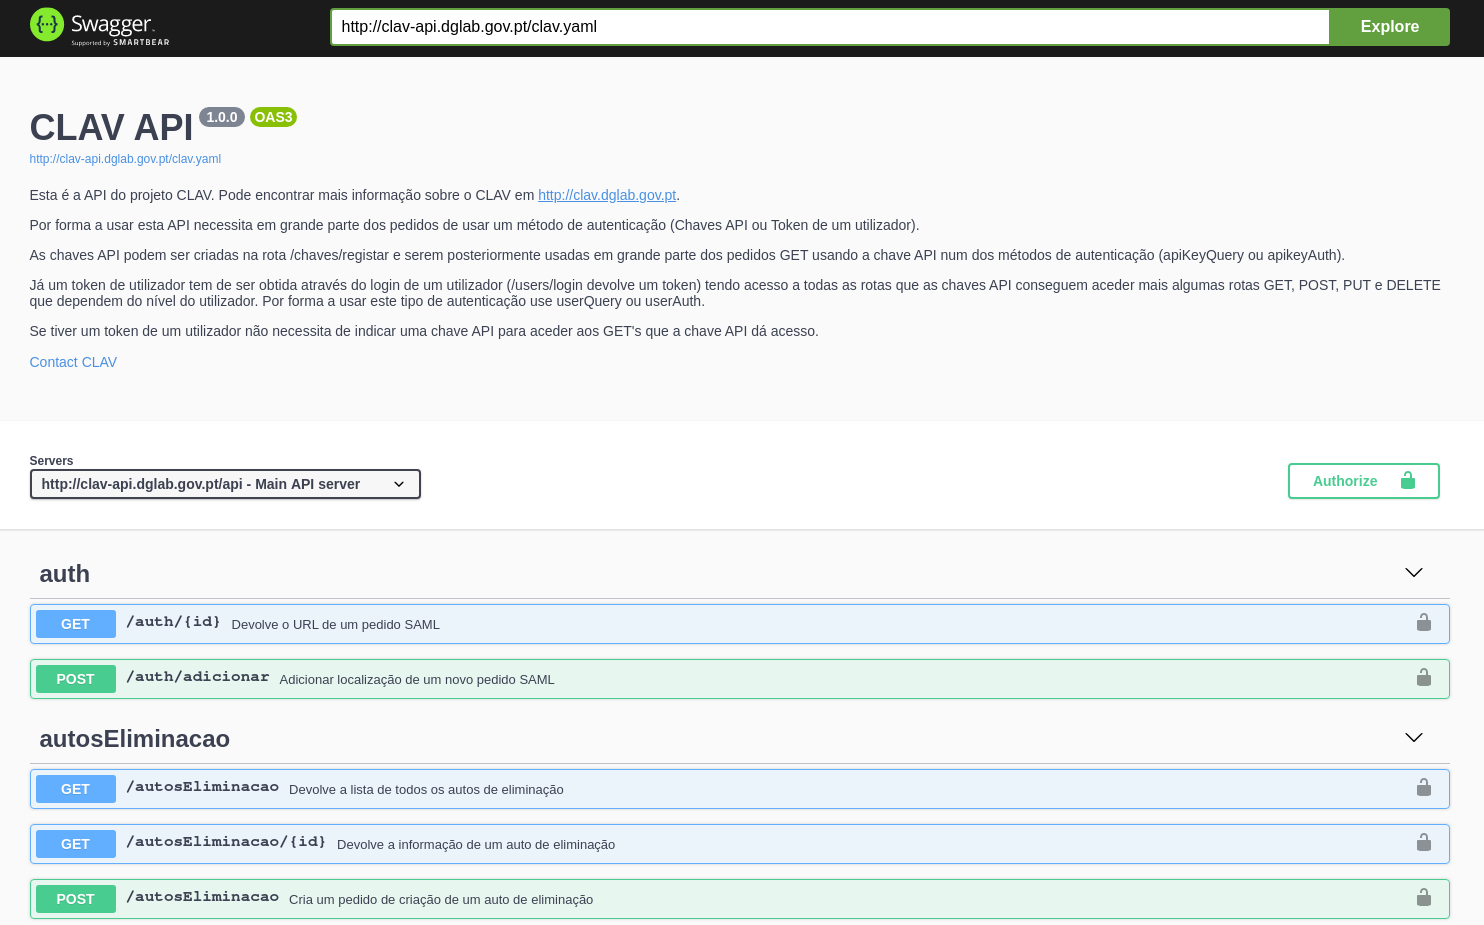
\includegraphics[width=0.5\textwidth]{img/swaggerUI.png}
    \end{center}
    \caption{\textit{Swagger \acrshort{ui}} exemplo}
\end{figure}

\subsubsection{Alternativas}
Existem várias alternativas ao \textit{Swagger \acrshort{ui}}:
\begin{savenotes}
\begin{table}[H]
    \footnotesize
    \begin{center}
    \begin{tabular}{|r|p{0.39\textwidth}|p{0.39\textwidth}|}
    \hline
    Ferramenta & Vantagens & Desvantagens \\ \hline
        \textit{Swagger \acrshort{ui}} &
        \begin{itemize}[leftmargin=0.3cm]
            \setlength\itemsep{0em}
            \item Suporta a especificação \textit{OpenAPI}
            \item \textit{Open-source}
            \item Amplamente usado
        \end{itemize}
        &
        %\begin{itemize}[leftmargin=0.3cm]
        %    \setlength\itemsep{0em}
        %    \item
        %\end{itemize}
        \\ \hline
    \textit{Apiary}\footnote{Ver \url{https://apiary.io/}} &
        \begin{itemize}[leftmargin=0.3cm]
            \setlength\itemsep{0em}
            \item Suporta a especificação \textit{\acrshort{api} Blueprint} e a especificação \textit{OpenAPI}
        \end{itemize}
        &
        \begin{itemize}[leftmargin=0.3cm]
            \setlength\itemsep{0em}
            \item Necessário pagar de forma a puder integrar a documentação da \acrshort{api} num domínio próprio
            \item \textit{Closed-source}
        \end{itemize}
        \\ \hline
    \textit{\acrshort{api} Console}\footnote{Ver \url{https://github.com/mulesoft/api-console}} &
        \begin{itemize}[leftmargin=0.3cm]
            \setlength\itemsep{0em}
            \item Suporta a especificação \acrshort{raml} e a especificação \textit{OpenAPI}
            \item \textit{Open-source}
        \end{itemize}
        &
        %\begin{itemize}[leftmargin=0.3cm]
        %    \setlength\itemsep{0em}
        %    \item
        %\end{itemize}
        \\ \hline
    \textit{Slate}\footnote{Ver \url{https://github.com/slatedocs/slate}} &
        \begin{itemize}[leftmargin=0.3cm]
            \setlength\itemsep{0em}
            \item \textit{Open-source}
            \item \acrshort{api} definida em \textit{Markdown}
        \end{itemize}
        &
        \begin{itemize}[leftmargin=0.3cm]
            \setlength\itemsep{0em}
            \item Não suporta nenhuma especificação
        \end{itemize}
        \\ \hline
    \textit{apiDoc}\footnote{Ver \url{https://apidocjs.com/}} &
        \begin{itemize}[leftmargin=0.3cm]
            \setlength\itemsep{0em}
            \item Documentação criada a partir das anotações nos comentários do código
            \item \textit{Open-source} 
        \end{itemize}
        &
        \begin{itemize}[leftmargin=0.3cm]
            \setlength\itemsep{0em}
            \item Não suporta nenhuma especificação
        \end{itemize}
        \\ \hline
    \textit{ReDoc}\footnote{Ver \url{https://github.com/Redocly/redoc}} &
        \begin{itemize}[leftmargin=0.3cm]
            \setlength\itemsep{0em}
            \item Suporta a especificação \textit{OpenAPI}
            \item \textit{Open-source} 
            \item Fácil de integrar
        \end{itemize}
        &
        %\begin{itemize}[leftmargin=0.3cm]
        %    \setlength\itemsep{0em}
        %    \item
        %\end{itemize}
        \\ \hline
    \end{tabular}
    \end{center}
    \caption{Comparação entre ferramentas de \acrshort{api}s}
\end{table}
\end{savenotes}

De forma a escolher a ferramenta apropriada é necessário ter em conta que:
\begin{itemize}
    \item Não há financiamento
    \item Já existe uma \acrshort{api} desenvolvida
    \item A documentação deve estar acessível de um domínio próprio
    \item A documentação deve ser fácil de criar, de editar e de manter
    \item Será usada a especificação \textit{OpenAPI}
\end{itemize}

As escolhas ficam como tal reduzidas ao \textit{Swagger \acrshort{ui}} e ao \textit{ReDoc}. Optou-se por escolher o \textit{Swagger \acrshort{ui}} visto ser a ferramenta mais amplamente usada para além de que é possível obter também uma fácil integração no \textit{Swagger \acrshort{ui}} com recurso à package \texttt{swagger-ui-express} que falaremos na próxima secção.

\section{Documentação da \acrshort{api} da \acrshort{clav}}

Agora sabendo que será usada a especificação \textit{OpenAPI} e o \textit{Swagger \acrshort{ui}} é importante perceber que bibliotecas devem ser usadas para a produção da documentação. 

Existem duas \textit{packages} que podem ser usadas para criar documentação interativa para uma \acrshort{api} \acrshort{rest} criada com \textit{Node.js} e \textit{Express.js}:~\cite{swaggerNode}
\begin{itemize}
    \item \texttt{swagger-node-express}
    \begin{itemize}
        \item Vantagens
        \begin{itemize}
            \item Módulo oficial suportado pelo \textit{Swagger}
            \item É \textit{open-source} e como tal é possível contribuir para a correção de problemas
            \item A solução contém \textit{Swagger Editor} e \textit{Swagger Codegen} e como tal tanto podemos usar uma abordagem \textit{top-down} como \textit{bottom-up}
        \end{itemize}
        \item Desvantagens
        \begin{itemize}
            \item Instalação manual do \textit{Swagger \acrshort{ui}}. O código do \textit{Swagger \acrshort{ui}} tem de ser copiado manualmente para o projeto e sempre que há uma atualização é necessário copiar novamente manualmente
            \item Instalação complexa. Por forma a aplicação hospedar a documentação é necessário adicionar algumas rotas ao servidor para além das já definidas na especificação \textit{OpenAPI}
            \item Fraca documentação
        \end{itemize}
    \end{itemize}
    \item \texttt{swagger-ui-express}
    \begin{itemize}
        \item Vantagens
        \begin{itemize}
            \item É \textit{open-source} e como tal é possível contribuir para a correção de problemas
            \item Não é necessário copiar manualmente o \textit{Swagger \acrshort{ui}}
            \item De fácil instalação, apenas é necessário adicionar uma rota aonde estará hospedada a documentação
            \item Boa documentação
        \end{itemize}
        \item Desvantagens
        \begin{itemize}
            \item Não é o módulo oficial suportado pelo \textit{Swagger}
        \end{itemize}
    \end{itemize}
\end{itemize}

Das duas foi escolhida a \texttt{swagger-ui-express} visto ser de mais simples implementação e de mais fácil manutenção.

\begin{lstlisting}[language=javascript, caption=Exemplo de uso do \texttt{swagger-ui-express}, label=exem:suie]
var swaggerUI = require('swagger-ui-express')
//JSON
var swaggerDocument = require('./swagger.json')
//ou YAML
var yaml = require('js-yaml')
var fs = require('fs')
var swaggerDocument = yaml.load(fs.readFileSync('./swagger.yaml'))

app.use('/doc', swaggerUI.serve, swaggerUI.setup(swaggerDocument));
\end{lstlisting}

No exemplo~\ref{exem:suie} a documentação da \acrshort{api} está presente na rota \texttt{'/doc'}. Neste exemplo é exemplificado como carregar uma especificação \textit{OpenAPI} em \acrshort{json} bem como em \acrshort{yaml}. Quanto ao \textit{middleware} \texttt{serve} retorna os ficheiros estáticos necessários para hospedar o \textit{Swagger \acrshort{ui}}. Já o segundo \textit{middleware} \texttt{setup} para além de puder receber o documento com a especificação \textit{OpenAPI} pode também receber um outro parâmetro de opções que o utilizador pode definir para a apresentação interativa da documentação com o \textit{Swagger \acrshort{ui}}\footnote{As opções possíveis estão presentes em \url{https://github.com/scottie1984/swagger-ui-express}. Para o atributo (opção) \texttt{swaggerOptions} as opções possíveis estão presentes em \url{https://github.com/swagger-api/swagger-ui/blob/master/docs/usage/configuration.md}}.

Agora há duas abordagens possíveis de realizar a documentação:
\begin{itemize}
    \item Documentação de cada rota nos comentários da rota através da utilização da \textit{package} \texttt{swagger-jsdoc}\footnote{Ver \url{https://github.com/Surnet/swagger-jsdoc}}
    \item Documentação à parte do código
\end{itemize}

A abordagem escolhida foi a da documentação à parte do código por forma a modularizar a documentação. A modularização da documentação foi realizada através do uso da \textit{package} \texttt{yaml-include}\footnote{Ver \url{https://github.com/claylo/yaml-include}}. Esta \textit{package} permite que o documento \acrshort{yaml} da especificação \textit{OpenAPI} possa ser dividida por vários ficheiros para além do que já é permitido através do \verb|$ref| da especificação \textit{OpenAPI}. Ela permite a inclusão de arquivos \acrshort{yaml} externos ou a inclusão de pastas de ficheiros \acrshort{yaml}. Esta funcionalidade é desaprovada pela equipa de desenvolvimento do \acrshort{yaml} contudo é de grande ajuda e de simplificação da construção do ficheiro de especificação \textit{OpenAPI}.

\begin{lstlisting}[language=yaml, caption=Exemplo de uso do \texttt{yaml-include} no documento de especificação \textit{OpenAPI}(\textit{index.yaml}), label=exem:yamli]
openapi: 3.0.0
info:
  description: Esta é a API do projeto CLAV. Pode encontrar mais informação sobre o CLAV em [http://clav.dglab.gov.pt](http://clav.dglab.gov.pt).
  version: 1.0.0
  title: CLAV API
  contact:
    name: CLAV
    email: clav@dglab.gov.pt
servers:
  - url: http://localhost:7779/api
    description: Local API server
paths: !!inc/dir [ 'paths' ]
components:
  schemas: !!inc/dir [ 'schemas', excludeTopLevelDirSeparator: true ]
  securitySchemes: !!inc/file '/security/schemes.yaml'
\end{lstlisting}

O ficheiro \textit{index.yaml} será a raiz do documento de especificação \textit{OpenAPI} a ser gerado com a \textit{package} \texttt{yaml-include}. A estrutura dos ficheiros para gerar o documento de especificação \textit{OpenAPI} final exemplifica como se pode dividir a documentação por vários ficheiros com esta \textit{package}:
\begin{lstlisting}[language=pseudocode, caption=Exemplo de estrutura dos ficheiros para gerar o documento de especificação \textit{OpenAPI}, label=exem:faf]
* index.yaml
* paths/
    * classes/
        * get.yaml
        * ~id/
            * get.yaml
    * users/
        * ~id/
            * post.yaml
            * delete.yaml
* schemas/
    * User.yaml
* security/
    * schemes.yaml
\end{lstlisting}

Assim, o \texttt{!!inc/dir} fará que no ficheiro \textit{index.yaml} na \textit{tag} \textit{paths} sejam incluídos todos os ficheiros que estão na pasta \textit{paths}. Cada ficheiro corresponderá a uma determinada rota com um determinado método \acrshort{http}. O método \acrshort{http} é definido a partir do nome do ficheiro e o caminho da rota é determinado pelo nome das pastas e do aninhamento destas. Quando o nome da pasta é iniciado por ``\verb|~|'' no caminho será colocado o nome da pasta sem o til entre chavetas (``\{\}'') por forma a indicar um parâmetro que é colocado no caminho do pedido.

Já no caso do \texttt{!!inc/dir} dos \textit{schemas} a opção \texttt{excludeTopLevelDirSeparator} permite que os ficheiros que estejam dentro da pasta \textit{schemas} (mas não aninhados dentro de outras pastas) sejam incluídos sem qualquer aninhamento, assumindo o nome do ficheiro como o atributo a colocar.

Existe também o \texttt{!!inc/file} que permite incluir sobe uma determinada \textit{tag} a informação presente no ficheiro referenciado pelo caminho.

O documento de especificação \textit{OpenAPI} final gerado será:
\begin{lstlisting}[language=yaml, caption=Documento de especificação \textit{OpenAPI} gerado a partir do ficheiro \textit{index.yaml} com o uso da \textit{package} \texttt{yaml-include}, label=exem:yamlif]
openapi: 3.0.0
info:
  description: Esta é a API do projeto CLAV. Pode encontrar mais informação sobre o CLAV em [http://clav.dglab.gov.pt](http://clav.dglab.gov.pt).
  version: 1.0.0
  title: CLAV API
  contact:
    name: CLAV
    email: clav@dglab.gov.pt
servers:
  - url: http://localhost:7779/api
    description: Local API server
paths:
  /classes:
    get:
      <conteúdo do ficheiro paths/classes/get.yaml>
  /users/{id}:
    post:
      <conteúdo do ficheiro paths/~id/post.yaml>
    delete:
      <conteúdo do ficheiro paths/~id/delete.yaml>
components:
  schemas:
    User:
      <conteúdo do ficheiro schemas/User.yaml>
  securitySchemes:
    <conteúdo do ficheiro security/schemes.yaml>
\end{lstlisting}

No final teremos um ficheiro no formato \acrshort{yaml} com toda a documentação da \acrshort{api} que puderá então ser usado para alimentar a documentação dinâmica \textit{Swagger \acrshort{ui}}.

%TODO
%\section{Importação de dados}
%TODO: falar da tabela de seleção

\section{Exportação de dados}

Esta tese tem como um dos objetivos a exportação de dados da \acrshort{api} de Classes, Entidades, Tipologias e Legislações em formato \acrshort{json}, \acrshort{xml} e \acrshort{csv}. Além disso, deve permitir a exportação da ontologia (possuidor da informação das variantes referidas a exportar) nos formatos \acrshort{turtle}, \acrshort{json-ld} e \acrshort{rdf}/\acrshort{xml}.

A \acrshort{api} de dados já devolve a sua informação em \acrshort{json}. Portanto, por forma a realizar a exportação dos dados para outros formatos é necessário realizar a conversão de \acrshort{json} para o formato de saída pretendido. Como tal, nesta secção será aprofundada algumas bibliotecas disponíveis no \acrshort{npm} que têm como objetivo exportar de \acrshort{json} para \acrshort{xml} ou de \acrshort{json} para \acrshort{csv}. É por fim, investigado como poderá ser exportada a ontologia a partir do GraphDB.

\subsection{\acrshort{xml}}

Comecemos por perceber o que é o \acrfull{xml}. Como se pode perceber pelo nome o \acrshort{xml} é uma linguagem \textit{Markup}, ou seja, uma linguagem que anota o texto para que a máquina possa manipular o texto de acordo com as anotações. O \acrshort{xml} foi desenhado para ser de fácil leitura tanto para humanos como para máquinas e tem como principal intuito o armazenamento e transporte de informação (o tal texto anotado). Além disso é extensível visto que permite que criemos as nossas tags.

\begin{lstlisting}[language=xml, caption=Pequeno exemplo em \acrshort{xml}, label=exem:xmlEx]
<?xml version = "1.0" encoding = "UTF-8"?>
<pessoa>
    <nome>Maria</nome>
    <idade tipo="numero">23</idade>
    <morada>
        <pais>Portugal</pais>
        <cidade>Braga</cidade>
    </morada>
    <altura unidade="cm">160</altura>
    <!--Isto é um comentário-->
</pessoa>
\end{lstlisting}

De seguida serão apresentadas, de forma simplificada, as regras de sintaxe aplicadas ao \acrshort{xml} para cada componente deste.

\begin{itemize}
    \item \textbf{Declaração \acrshort{xml}} \\
    \verb|<?xml version = "1.0" encoding = "UTF-8"?>| \\
    Opcional, especifica a versão do \acrshort{xml} e o encoding usado no documento
    \begin{itemize}
        \item A declaração é \textit{case-sensitive} pelo que deve começar obrigatoriamente por \texttt{xml}
        \item Se presente no documento, a declaração tem de ser obrigatoriamente o primeiro componente
    \end{itemize}
    \item \textbf{Tags e elementos} \\
    \verb|<nome>Maria</nome>| ou \verb|<semnome/>|
    \begin{itemize}
        \item Cada elemento tem de ser fechado seja por uma tag (tag final), ou como apresentado acima pela própria tag.
        \item Os elementos \acrshort{xml} podem conter elementos filhos mas estes não se podem sobrepor, ou seja, uma tag final de um elemento tem de ter o mesmo nome que a última tag inicial ainda sem tag final. 
        \item Um documento \acrshort{xml} apenas pode ter um elemento na raíz do documento (elemento \textit{root})
        \item Os nomes das tags são \textit{case-sensitive}, portanto, a tag inicial e final de um elemento tem de ser exatamente iguais
    \end{itemize}
    \item \textbf{Atributos} \\
    \verb|<altura unidade="cm">160</altura>| \\
    onde `unidade' é o nome do atributo e `cm' é o valor do atributo. Um atributo especifica uma propriedade de um elemento
    \begin{itemize}
        \item Um elemento pode ter zero, um ou mais atributos
        \item Os nomes dos atributos são \textit{case-sensitive}
        \item Um atributo não pode ter dois valores num elemento, ou seja, não pode ser declarado duas ou mais vezes num mesmo elemento
        \item Os nomes dos atributos não podem possuir aspas, mas os valores tem de ser encapsolados por aspas
    \end{itemize}
    \item \textbf{Referências \acrshort{xml}} \\
    \verb|&amp;| ou \verb|&#65| \\
    Há dois tipos de referências, Referências Entidade ou Referências Caractere. A primeira existe por forma a serem representadas por estas referências os caracteres não permitidos no texto anotado visto representarem parte da sintaxe do \acrshort{xml}.
    \begin{center}
        \begin{tabular}{|c|c|}
            \hline
            Caractere não permitido & Entidade \\ \hline
            < & \&lt; \\ \hline
            > & \&gt; \\ \hline
            \& & \&amp; \\ \hline
            ' & \&apos; \\ \hline
            " & \&quot; \\ \hline
        \end{tabular}
    \end{center}
    O segundo tipo de referências tem o mesmo intuito mas permite que seja representado qualquer caractere representável em \textit{Unicode}. O número que se segue ao hashtag é referente ao código decimal em \textit{Unicode}. Assim \verb|&#65| representa o caractere `A'.
    \item \textbf{Texto anotado} \\
    Espaços em branco, tabs, ou novas linhas, são ignoradas quando presentes entre elementos e entre atributos. Como já referido há caracteres reservados pelo que se pretende usá-los no texto anotado deve trocar esses caracteres pelas suas referências.
\end{itemize}

\subsubsection{Bibliotecas de conversão}

Nesta secção serão abordadas algumas bibliotecas de conversão de \acrshort{json} para \acrshort{xml}, aquelas com maior popularidade e adesão no \acrshort{npm}.

Por forma a ter uma ideia do resultado devolvido por cada biblioteca será usado o seguinte exemplo:
\begin{lstlisting}[language=json, caption=Exemplo em \acrshort{json} a converter, label=exem:jsonBib]
[
    {
        "nome": "Maria",
        "idade": "22",
        "morada": {
            "pais": "Portugal",
            "cidade": "Braga"
        }
    },
    {
        "nome": "João",
        "idade": "24",
        "morada": {
            "pais": "Portugal",
            "cidade": "Vila Real"
        }
    }
]
\end{lstlisting}

\paragraph{\href{https://www.npmjs.com/package/xml-js}{\texttt{xml-js}}} \mbox{} \\

Esta biblioteca permite a conversão nos dois sentidos, ou seja, de \acrshort{json} para \acrshort{xml} e de \acrshort{xml} para \acrshort{json}.

As principais características que esta biblioteca possui para uma conversão de \acrshort{json} para \acrshort{xml} são:
\begin{itemize}
    \item Mantém a ordem dos elementos
    \item Totalmente compatível com \acrshort{xml}
    \item Reversível, é possível reverter o resultado para o original
    \item Podem ser fornecidas funções personalizadas para processamento adicional para diferentes partes do \acrshort{xml} ou do \acrshort{json} a converter
\end{itemize}

\begin{lstlisting}[language=xml, caption=Resultado da conversão do exemplo~\ref{exem:jsonBib} usando o conversor \texttt{xml-js}]
<0>
    <nome>Maria</nome>
    <idade>22</idade>
    <morada>
        <pais>Portugal</pais>
        <cidade>Braga</cidade>
    </morada>
</0>
<1>
    <nome>João</nome>
    <idade>24</idade>
    <morada>
        <pais>Portugal</pais>
        <cidade>Vila Real</cidade>
    </morada>
</1>
\end{lstlisting}

\paragraph{\href{https://www.npmjs.com/package/xmlbuilder}{\texttt{xmlbuilder}}} \mbox{} \\

A biblioteca tem como intuito principal a construção de documentos \acrshort{xml} através do uso de funções, como se pode comprovar de seguida:

\begin{lstlisting}[language=javascript, caption=Código para a construção em \acrshort{xml} do exemplo~\ref{exem:xmlEx} usando o \texttt{xmlbuilder}]
var builder = require('xmlbuilder');
 
var xml = builder.create('pessoa')
    .ele('nome', 'Maria')
    .up()
    .ele('idade', {'tipo': 'numero'}, '23')
    .up()
    .ele('morada')
    .ele('pais', 'Portugal')
    .up()
    .ele('cidade', 'Braga')
    .up()
    .up()
    .ele('altura', {'unidade': 'cm'}, '160')
    .up()
    .com('Isto é um comentário')
    .end({ pretty: true});
\end{lstlisting}

Além disso, permite a geração do \acrshort{xml} a partir de um objeto \acrshort{json} o que permite, como tal, a conversão de \acrshort{json} para \acrshort{xml} que se necessita.

\begin{lstlisting}[language=xml, caption=Resultado da conversão do exemplo~\ref{exem:jsonBib} usando o conversor \texttt{xmlbuilder}]
<?xml version="1.0" encoding="utf-8"?>
<nome>Maria</nome>
<idade>22</idade>
<morada>
  <pais>Portugal</pais>
  <cidade>Braga</cidade>
</morada>
<nome>João</nome>
<idade>24</idade>
<morada>
  <pais>Portugal</pais>
  <cidade>Vila Real</cidade>
</morada>
\end{lstlisting}

Na construção do documento a partir de um objecto, quando se pretende que um elemento tenha um atributo, é necessário que o objeto para essa chave possua um objeto em vez de apenas o valor. Nesse objeto, as propriedades começadas por `@' indicam atributos (\verb|'@unidade':'cm'| onde `unidade' é o nome do atributo e `cm' é o valor do atributo) e a propriedade '\#text' representa o valor do elemento.

Há também a possibilidade de sobescrever as funções usadas para escrever o documento \acrshort{xml} (funções de escrita dos elementos, comentários, etc) bem como as funções que convertem os valores (texto anotado, nome de elementos e atributos, etc).

Por fim, convém referir que esta biblioteca já possui uma sucessora, \href{https://www.npmjs.com/package/xmlbuilder2}{\texttt{xmlbuilder2}}, que foi redesenhada por forma a estar em total conformidade com a especificação moderna do \acrshort{dom}.

\paragraph{\href{https://www.npmjs.com/package/xml2js}{\texttt{xml2js}}} \mbox{} \\

De igual forma como a biblioteca \texttt{xml-js}, esta biblioteca consegue converter de \acrshort{json} para \acrshort{xml} como de \acrshort{xml} para \acrshort{json}. 

\begin{lstlisting}[language=xml, caption=Resultado da conversão do exemplo~\ref{exem:jsonBib} usando o conversor \texttt{xml2js}]
<?xml version="1.0" encoding="UTF-8" standalone="yes"?>
<root>
  <nome>Maria</nome>
  <idade>22</idade>
  <morada>
    <pais>Portugal</pais>
    <cidade>Braga</cidade>
  </morada>
  <nome>João</nome>
  <idade>24</idade>
  <morada>
    <pais>Portugal</pais>
    <cidade>Vila Real</cidade>
  </morada>
</root>
\end{lstlisting}

Se se pretende que um determinado elemento possua atributos é necessário que o objeto para esse elemento seja um objeto (\verb|{$: {unidade: 'cm'}, _: '160'}|) onde `\_' é o texto anotado e os vários atributos devem estar no objeto da propriedade `\$' em que o nome da propriedade é o nome do atributo e o valor da propriedade e o valor do atributo.

\subsection{\acrshort{csv}}

\acrfull{csv} como o seu acrónimo indica é um documento em que os campos de um registo são separados por uma vírgula. Contudo, os campos não precisam de ser obrigatoriamente separados por vírgula já que podem também ser separados por ponto e vírgula, tabs, pipes (`|') ou ainda outro qualquer caractere que se pretenda usar. Quando se usa o caractere separador ou uma nova linha (`\backslash{}n') no campo de um registo, por forma a não ser considerado como um separador de campos ou de registos respetivamente, pode-se encapsolar os valores por aspas (`"') sendo que também se pode usar outro caractere em vez das aspas. Já quando se usa o caractere de encapsolamento no campo de um registo este deve ser protegido (\texttt{escaped}) repetindo o mesmo caractere de encapsolamento.

Um documento \acrshort{csv} é nada mais que uma tabela que guarda dados em texto. É usado essencialmente para a troca de dados.

Após esta pequena introdução ao \acrshort{csv} apresenta-se as regras de sintaxe para a criação de um documento \acrshort{csv}:
\begin{itemize}
    \item Campos separados com um separador, normalmente uma vírgula
    \item Cada registo deve estar numa linha. Cada registo deve começar numa linha, mas cada registo pode ter várias linhas, desde que os campos multi linha sejam encapsolados por aspas
    \item Após o último registo não deve estar presente um \textit{carriage return}
    \item Opcionalmente, na primeira linha do documento, deve estar presente o cabeçalho com os nomes das colunas separados pelo separador usado no resto do documento
    \item O caractere de encapsolamente deve ser usado para encapsolar um campo quando necessário (pode ser usado sempre), isto é, quando o caractere separador ou uma nova linha (`\backslash{}n') são usados num campo de um registo
\end{itemize}

\begin{lstlisting}[caption=Pequeno exemplo em \acrshort{csv}, label=exem:csvEx]
Nome,Idade,País,Cidade,Altura
"Silva, Maria",23,Portugal,Braga,160cm
\end{lstlisting}

\subsubsection{Bibliotecas de conversão}

Nesta secção irá também ser aprofundada algumas bibliotecas de conversão de \acrshort{json} para \acrshort{csv}, aquelas com maior popularidade no \acrshort{npm}.

\paragraph{\href{https://www.npmjs.com/package/papaparse}{\texttt{papaparse}}} \mbox{} \\

O \texttt{papaparse} tem como principal objetivo realizar o \textit{parse} de ficheiros \acrshort{csv}. Consegue contudo reverter, convertendo de \acrshort{json} para \acrshort{csv}.

\begin{lstlisting}[caption=Resultado da conversão do exemplo~\ref{exem:jsonBib} usando o conversor \texttt{papaparse}, label=exem:papaparse]
nome,idade,morada
Maria,22,[object Object]
João,24,[object Object]
\end{lstlisting}

Olhando para o resultado~\ref{exem:papaparse} consegue-se perceber que o conversor não consegue converter objetos aninhados. Para além disso, apesar de haver a possibilidade de alterar o caractere separador, o caracter de \textit{escape}, o caractere de nova linha bem como definir o nome das colunas no cabeçalho, não é possível definir uma função por forma a alterar a conversão dos campos de cada propriedade.

\paragraph{\href{https://www.npmjs.com/package/json2csv}{\texttt{json2csv}}} \mbox{} \\

Biblioteca totalmente dedicada à conversão de \acrshort{json} para \acrshort{csv}. Tem como principais características:
\begin{itemize}
    \item Permite a alteração dos carecteres de separação, de encapsolamento e de nova linha
    \item \textit{Escape} automático
    \item Permite escolher que campos devolver (mesmo em objetos aninhados ou listas aninhadas) e que cabeçalho associar a cada campo
    \item Aceita funções de transformação para cada campo
\end{itemize}

\begin{lstlisting}[caption=Resultado da conversão do exemplo~\ref{exem:jsonBib} usando o conversor \texttt{json2csv}, label=exem:json2csv]
"nome","idade","morada.pais","morada.cidade"
"Maria","22","Portugal","Braga"
"João","24","Portugal","Vila Real"
\end{lstlisting}

Para além disso permite o \textit{unwind} de uma propriedade que possua uma lista, fazendo com que sejam gerados x registos de acordo com o tamanho da lista, sendo alterado apenas os valores que proveem da lista. Infelizmente isto acrecenta mais colunas, não permitindo que no caso de os elementos da lista (filhos) tenham a mesma estrutura que o pai, sejam adicionados como novos registos, sem adicionar novas colunas e sem repetir a informação do pai. 

Por exemplo, se pretendermos converter o seguinte documento \acrshort{json}:
\begin{lstlisting}[language=json, caption=Outro exemplo em \acrshort{json} a converter, label=exem:jsonBib2]
[
    {
        "nome": "Maria",
        "idade": "22",
        "morada": {
            "pais": "Portugal",
            "cidade": "Braga"
        },
        "filhos": [
          {
            "nome": "António",
            "idade": "24",
            "morada": {
                "pais": "Portugal",
                "cidade": "Aveiro"
            }
          }
        ]
    },
    {
        "nome": "João",
        "idade": "24",
        "morada": {
            "pais": "Portugal",
            "cidade": "Vila Real"
        },
        "filhos": []
    }
]
\end{lstlisting}

Usando este conversor é possível obter:
\begin{lstlisting}[caption=Resultado da conversão do exemplo~\ref{exem:jsonBib2} usando o conversor \texttt{json2csv}]
"nome","idade","morada.pais","morada.cidade","filhos.nome","filhos.idade","filhos.morada.pais","filhos.morada.cidade"
"Maria","22","Portugal","Braga","António","2","Portugal","Braga"
"João","24","Portugal","Vila Real",,,,
\end{lstlisting}

Quando o resultado pretendido seria por exemplo:
\begin{lstlisting}[caption=Resultado pretendido da conversão do exemplo~\ref{exem:jsonBib2}]
"nome","idade","morada.pais","morada.cidade"
"Maria","22","Portugal","Braga",
"António","24","Portugal","Aveiro"
"João","24","Portugal","Vila Real"
\end{lstlisting}

\subsection{Exportação da Ontologia}

\subsubsection{O que é uma ontologia?}

Uma ontologia é uma descrição formal e explícita de conceitos num domínio de discurso (classes, chamado às vezes de conceitos), propriedades de cada conceito que descrevem várias características e atributos do conceito (slots, às vezes chamados de funções ou propriedades) e restrições sobre slots (facetas, às vezes chamadas de restrições de função).~\cite{ontologyProt} Uma ontologia, juntamente com um conjunto de instâncias individuais de classes, constitui uma base de conhecimento.~\cite{ontologyProt}

Uma ontologia pode ser dividida em duas partes:
\begin{itemize}
    \item Estrutura: Onde é definido as classes, as propriedades (slots) e as restrições das propriedades (facetas)
    \item População: Onde é definido indíviduos (de classes) e propriedades dos indíviduos. Esta parte é construída tendo por base a estrutura definída.
\end{itemize}
De certa forma, a estrutura é como se fosse o modelo definido e a população a informação guardada respeitando o modelo definido.

Falemos agora um pouco mais sobre cada componente de uma ontologia.

Começando pelas classes, estas correspondem a conceitos, sendo que uma classe pode ter subclasses (onde uma subclasse herda as propriedades da sua superclasse) e superclasses. Para além disso, as classes possuem instâncias (ou indivíduos). Quanto às propriedades das classes existem dois tipos:
\begin{itemize}
    \item Atributos: propriedade que permite definir uma característica de uma classe (ou indivíduo) (p.e: Se pessoa for uma classe, o nome será um atributo)
    \item Relações: propriedade que permite estabelecer relações entre classes (ou indivíduos) (p.e: A relação de pai entre duas pessoas) 
\end{itemize}

As próprias propriedades podem ser caracterizadas através das restrições. As principais restrições são:
\begin{itemize}
    \item Cardinalidade: Indica quantos valores pode ter uma propriedade, \texttt{0} a \texttt{n} (p.e: Uma pessoa só tem um pai biológico.; outro exemplo: Uma pessoa pode ter várias nacionalidades)
    \item Tipo de valor: Indica que tipo de valor terá a propriedade (atributo), \textit{string}, número, \textit{boolean}, etc (p.e: A idade de uma pessoa é um número; outro exemplo: O nome de uma pessoa é uma \textit{string})
    \item \textit{Domain} e \textit{Range}: Indica que tipo de instâncias podem ser relacionadas por uma propriedade. O \textit{Domain} indica a quem pertence a propriedade (atributo ou relação). Já o \textit{Range} indica para uma relação o tipo de instâncias que podem ser relacionadas com o \textit{Domain} (p.e: Na relação pai, o seu \textit{Domain} e o seu \textit{Range} são iguais a Pessoa.; outro exemplo: Seja Animal outra classe, a relação tem dono tem como \textit{Domain} Animal e como \textit{Range} Pessoa; ainda outro exemplo: O \textit{Domain} do atributo nome é Pessoa)
\end{itemize}

Existem várias linguagens de ontologia, contudo, quando se trata de informação semântica na \textit{Web}, destaca-se a família de especificações \acrfull{rdf}. É esta a usada pelo \textit{GraphDB} onde este usa o \acrfull{sparql} por forma a questionar as bases de dados, como protocolo e como linguagem para descrever as questões a realizar. O \acrshort{rdf} tem como ideia a criação de afirmações acerca de recursos em expressões do tipo \verb|sujeito predicado objeto|. Além disso o \acrshort{rdf} possui vários formatos de serialização tais como \acrshort{turtle}, N-Triples, N-Quads, \acrshort{json-ld}, \acrshort{n3}, \acrshort{rdf}/\acrshort{xml} e \acrshort{rdf}/\acrshort{json}.

%TODO
%\section{Web Semântica}
%~\cite{lsparql}

%TODO
%\subsection{RDF}
%~\cite{lsparql}

%TODO
%\subsection{SPARQL}
%~\cite{lsparql}

%TODO
%\section{GraphDB}
%procurar "semelhantes" para cada um (Neo4j)

\subsubsection{\textit{GraphDB}}

Por fim quanto à exportação da ontologia, das três é a mais simples visto que o \textit{GraphDB}\footnote{\acrfull{bd} Semântica baseada em grafos compatível com os padrões \acrshort{w3c}. Suporta \acrshort{rdf} e \acrshort{sparql}} possui funcionalidades de exportação dos triplos presentes numa \acrshort{bd} armazenada no \textit{GraphDB}.

Para um fácil uso e compatibilidade com os \textit{standards} da indústria, o \textit{GraphDB} implementou as interfaces da \textit{framework} \textit{RDF4J}, a especificação do protocolo \acrshort{w3c} \acrshort{sparql}\footnote{Ver \url{https://www.w3.org/TR/sparql11-protocol/}} e suporta vários formatos de serialização \acrshort{rdf}\footnote{\label{fnRDF}\textit{TriG}, \textit{BinaryRDF}, \textit{TriX}, \textit{N-Triples}, \textit{N-Quads}, \acrshort{n3}, \acrshort{rdf}/\acrshort{xml}, \acrshort{rdf}/\acrshort{json}, \acrshort{json-ld} e \acrshort{turtle}}.~\cite{graphdbAbout}

O \textit{GraphDB} é um \textit{plugin} \acrshort{sail} para a \textit{framework} \textit{RDF4J} fazendo uso extensivo dos recursos e infraestrutura do \textit{RDF4J} especialmente do modelo \acrshort{rdf}, dos \textit{parsers} \acrshort{rdf} e dos motores de pesquisa.~\cite{graphdbArch}

Assim, o \textit{GraphDB} possui uma \acrshort{rest} \acrshort{api} do servidor RDF4J\footnote{Ver \url{https://rdf4j.org/documentation/rest-api/}} a partir da qual é possível obter todos os triplos de uma \acrshort{bd} através da rota
\begin{verbatim}
<url do GraphDB>/repositories/<id do repositório (BD)>/statements
\end{verbatim}
indicando no cabeçalho \acrshort{http} \textit{Accept} o formato de serialização \acrshort{rdf}\footnoteref{fnRDF} de saída (\textit{\acrshort{mime} type}\footnote{\textit{Standard} que indica a natureza e o formato de um documento, ficheiro ou conjunto de \textit{bytes}. Ver \href{https://tools.ietf.org/html/rfc6838}{RFC 6838}}) dos triplos. Dos vários formatos de serialização \acrshort{rdf} serão apenas suportados (acessíveis) na \acrshort{clav}, como já indicado, o \acrshort{turtle} (\texttt{text/turtle}), o \acrshort{json-ld} (\texttt{application/ld+json}) e o \acrshort{rdf}/\acrshort{xml} (\texttt{application/rdf+xml}).

%TODO
%\section{Nginx}
%~\cite{nginxcook}
%procurar "semelhantes" para cada um

%TODO
%\section{Docker}
%~\cite{udocker}
%procurar "semelhantes" para cada um

%TODO
%\section{Docker Compose}
%~\cite{udocker}
%procurar "semelhantes" para cada um
